\documentclass[a4paper]{article}

\hoffset=-1in
\voffset=-1in
\textwidth=150mm
\textheight=200mm

\usepackage{amsmath}
\usepackage{graphicx}
\usepackage{multicol}

\begin{document}
    \begin{figure}
        \centering
        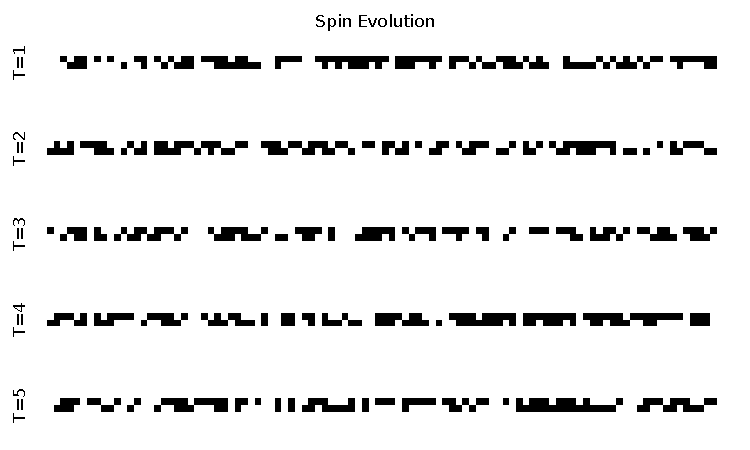
\includegraphics[width=0.5\textwidth]{pub/figures/q1a.pdf}
        \caption{At low temperatures we observed smaller groups of aligned %
            spins. We concluded that the influence of the heat (i.e. %
            \(\tau\sigma\)) on the free energy was low and therefore, that %
            the energy \(U\) was minmised.}
        \label{FIG1}
    \end{figure}

    Given the partition function \(Z = (2\cosh(\epsilon / \tau))^{N}\), we 
    calculated the internal energy using,
    %
    \begin{align}
\end{document}
